\chapter{A felhasználói felület}

Itt kellene majd bemutatni, hogy a felhasználói felület egyáltalán milyen részekből áll, azokat hogy lehet elérni és használni.

Attól függően, hogy a funkciók inkább kliens vagy szerver oldalon lesznek majd, itt lehet részletezni az összes, felhasználói felülettel kapcsolatos tudnivalót, de az is jó megoldás, ha minden funkciónál külön kerül bemutatásra.

\section{Felhasználói felület}

\subsection{Bejelentkezés/ regisztráció}

Az alkalmazás használatához érvényes felhasználói fiókra van szükség. Az alkalmazást használó felhasználókat két típusra lehet bontani, vannak az egyszerű userek(vásárlók), akik ételeket tudnak rendelni az adatbázisban szereplő éttermekből, és vannak az étteremtulajdonosok, akik saját éttermüket tudják menedzselni. Az alkalmazás további szolgáltatásainak az igénybevételéhez mindenképp be kell jelentkezni vagy userként, vagy étteremtulajdonosként. Amennyibben a felhasználó most először látogatott el az oldalra, és még nincs felhasználói fiókja, van lehetősége userként regisztrálnia magát. Ehhez mindössze egy egyszerű űrlapot kell kitöltenie, ahol többek között meg kell adnia a nevét, elérhetőségét, címét. Abban az esetben, ha valaki étteremtulajdonosként szeretne regisztrálni, meg kell keresni egy email-el az oldal üzemeltetőjét.

\begin{figure}
\centering
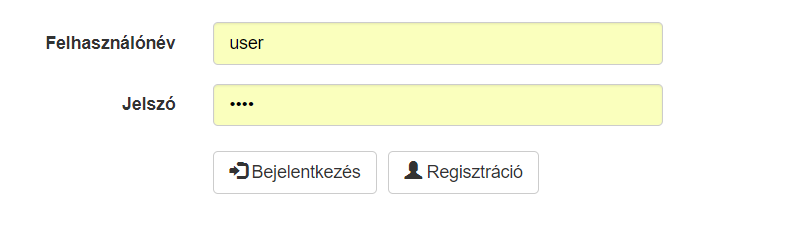
\includegraphics[scale=0.8]{kepek/login.png}
\caption{Bejelentkező felület}
\label{fig:architecture}
\end{figure}

\section{Egyszerű user funkciói}

A továbbiakban az alapfunkciókat a szerint fogom leírni, hogy melyik felhasználói csoport számára érhetők el. A vásárlók által elérhető szolgáltatásokkal kezdem

\subsection{Éttermek listázása}

A vásárlók számára adott egy olyan funkció, hogy ki tudják listázni az adatbázisban szereplő összes éttermet. Az éttermek egymás alatt, egy táblázatban jelennek meg. A táblázatban szerepel az étterem logója, neve, rövid leírása, címe, a várható kiszállítási idő, kiszállítási költség, a minimális rendelés összege és egy gomb, amire kattintva az oldal tovább irányítja a vásárlót az adott étterem étlapjához (\ref{fig:restaurants}. ábra).

A vásárlónak lehetősége van szűrni az éttermeket város szerint, ami segíti őket abban, hogy csak a számukra elérhető távolságban levő éttermek kínálatát lássák.

\begin{figure}
\centering
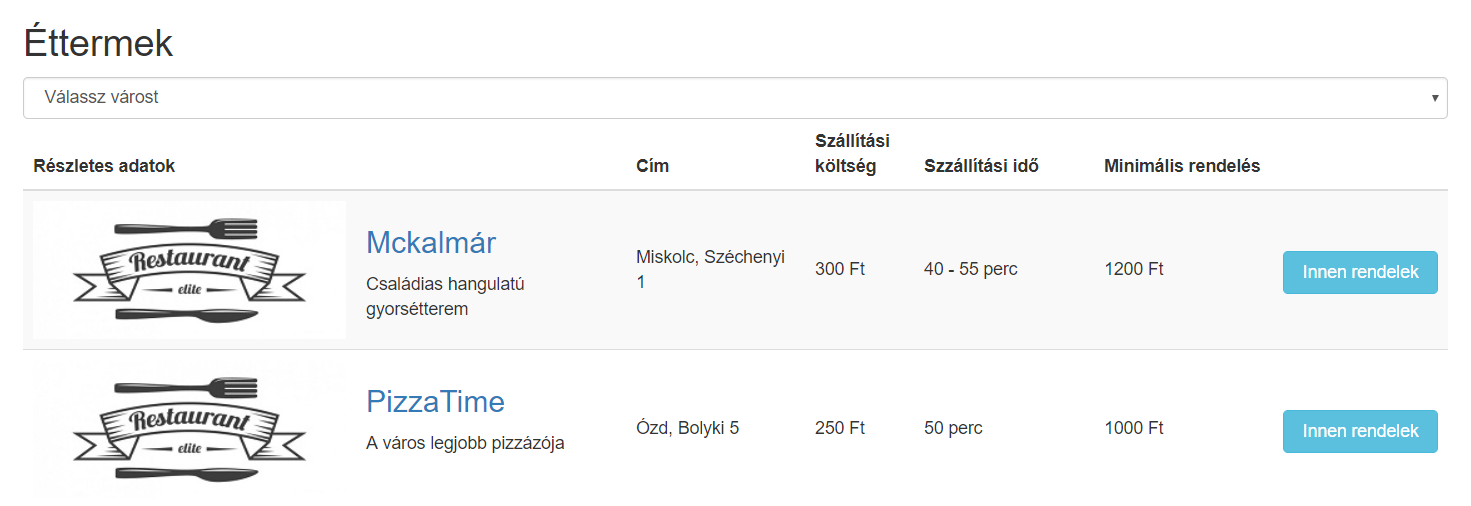
\includegraphics[scale=0.5]{kepek/restaurants.png}
\caption{Az éttermek listázása}
\label{fig:restaurants}
\end{figure}

\subsection{Étlap}

Miután a vásárló kiválasztotta a neki legszimpatikusabb éttermet, az „innen rendelek” gombra kattintva el lehet érni az adott étterem étlapját.

Az ételek egymás alatt, egy táblázatban jelennek meg (\ref{fig:menu}. ábra). A táblázat egyes soraiban egy-egy étel szerepel, az oszlopaiban pedig az adott étel adatai, többek között neve, egy kép róla, az ára és egy rövid leírás róla. A táblázat jobb szélső oszlopában egy „kosárba” feliratú gomb található, amit megnyomva a kiválasztott termék belekerül a felhasználó kosarába.

Az étlap felett van egy legördülő menü, ahol vásárló kiválaszthatja, hogy milyen típusú ételek között szeretne válogatni, milyen típusút szeretne rendelni. Az étel típus kiválasztása után, az ételek listája szűrve lesz az adott típus szerint, tehát csak a kívánt típusú ételek fognak megjelenni a táblázatban.

Miután a vásárló kiválasztotta a rendelni kívánt termékeket, és hozzáadta őket a kosárhoz, megjelenik a felületen a „fizetés” gomb, amire kattintva elérjük a fizetés funkciót.

\begin{figure}
\centering
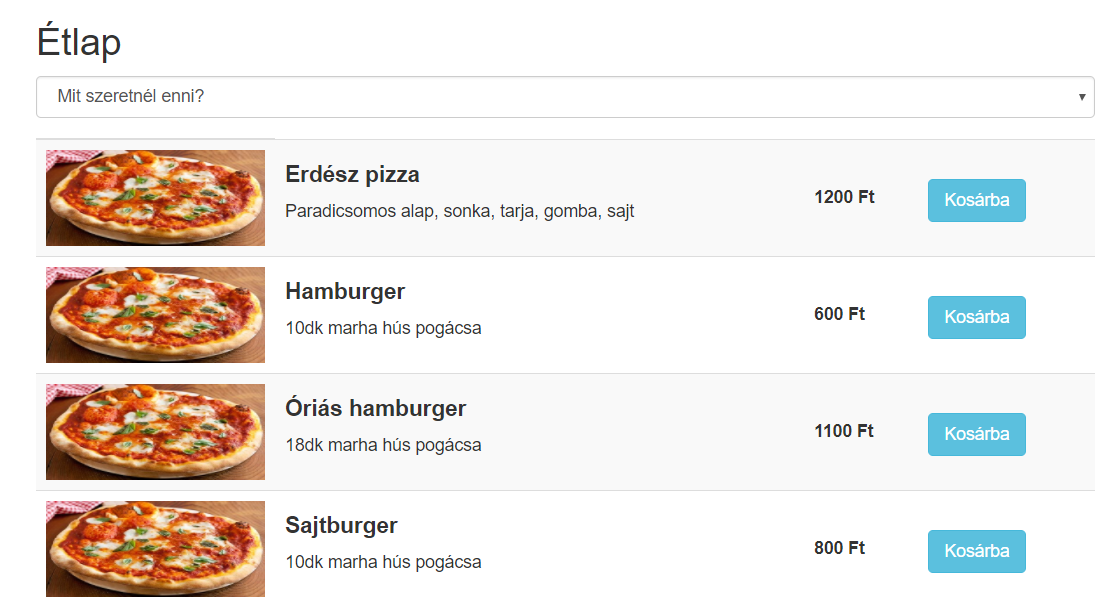
\includegraphics[scale=0.5]{kepek/menu.png}
\caption{Kép egy, az alkalmazásban megjelenített étlapról}
\label{fig:menu}
\end{figure}

\subsection{Fizetés}

A felhasználói felületen a kosár az étlap mellett, jobb oldalon található szintén egy táblázatos megoldással. A hozzáadott termékek neve és ára egymás alatt jelenik meg, egy végösszeggel a táblázat alján (\ref{fig:order}. ábra).

A kosár legalsó sorában egy „fizetés” gomb található. A gombra kattintva felugrik egy modal ablak, ahol egy legördülő menüből lehet kiválasztani a kívánt fizetési módot. Az alkalmazásban korlátozott számú fizetési lehetőség van, ami éttermenként változó lehet. Hogy egy étterem milyen fizetési lehetőségeket biztosít, azt az adott étterem felvitelekor kell megadni.

\begin{figure}
\centering
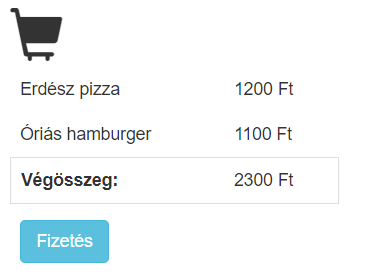
\includegraphics[scale=0.8]{kepek/order.png}
\caption{A vásárlás tételei összeggel és végösszeggel megjelenítve}
\label{fig:order}
\end{figure}

A kívánt fizetési lehetőség kiválasztása után (\ref{fig:payment}. ábra) a fizetés gombbal lehet véglegesíteni a megrendelést. Ilyenkor kapunk értesítést, hogy sikeres volt a rendelés.

\begin{figure}
\centering
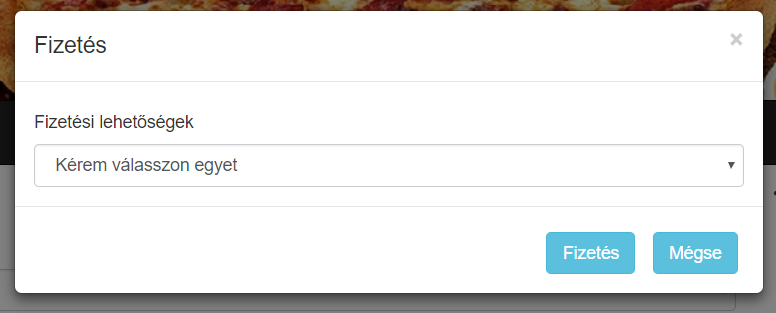
\includegraphics[scale=0.8]{kepek/payment.png}
\caption{A fizetési mód kiválasztása}
\label{fig:payment}
\end{figure}

\subsection{Profilom}

A profilom funkció kilistázza a bejelentkezett felhasználó adatait. Egy táblázatba foglalva kilistázza a felhasználó teljes nevét, felhasználónevét, email címét, telefonszámát, jutalompontját és címét/címeit. Egy felhasználónak akár több különböző szállítása címe is. A táblázat legalsó sorában van egy gomb „jelszó módosítása” felirattal (\ref{fig:profile}. ábra).

Jutalompontot a rendelések után kap a vásárló, minden elköltött 100 forint után egy jutalom pontot ír jóvá a rendszer. Az összegyűjtött pontokat, fizetéskor be lehet váltani, ilyenkor a beváltott pontok összege levonásra kerül a rendelés végösszegéből.

\begin{figure}
\centering
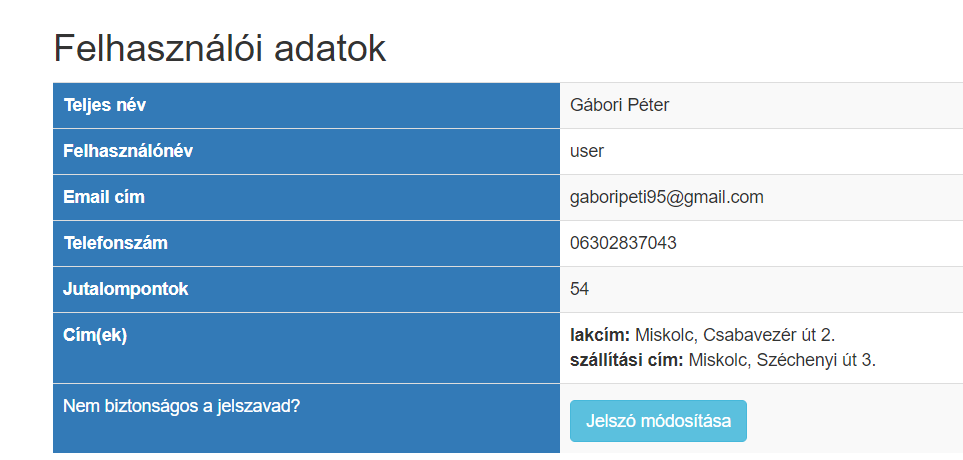
\includegraphics[scale=0.6]{kepek/profile.png}
\caption{Felhasználói adatok megjelenítése}
\label{fig:profile}
\end{figure}

A „Jelszó módosítása” gombra kattintva megjelenik egy űrlap, ahol a felhasználónak lehetősége van megváltoztatni a jelenlegi jelszavát (\ref{fig:password}. ábra). Meg kell adnia a jelenlegi jelszavát, majd az új jelszavát és végül meg kell erősítenie az új jelszót. Ha kitöltötte a bemeneti mezőket, a „Mentés” gombra kattintva megtörténik a jelszó cserélő funkció meghívása. Amennyibben a jelenlegi jelszó helyes, az új jelszó megfelel a kritériumoknak és megegyezik a megerősített jelszóval, megtörténik a jelszó módosítása.

\begin{figure}
\centering
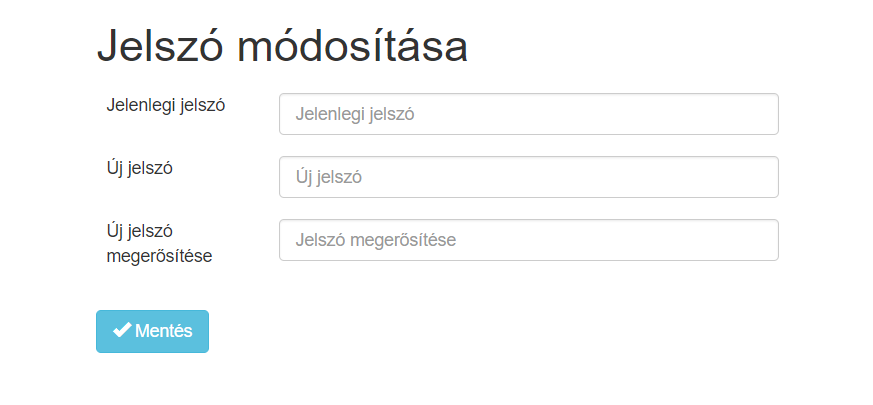
\includegraphics[scale=0.8]{kepek/password.png}
\caption{Jelszó megváltoztatása}
\label{fig:password}
\end{figure}

\section{Étterem tulajdonos funkciók}

\subsection{Éttermeim}

Az éttermeim funkció kilistázza a felhasználó adatbázisban szereplő éttermeit. Az éttermek táblázatos elrendezésben jelennek meg a felületen, a táblázat minden egyes sora, egy éttermet reprezentál. A táblázat oszlopaiban az éttermek különböző adatai találhatók, többek között az étterem logója, neve címe. A jobb szélső oszlopban három gomb található, „Étlap szerkesztése”, „Étterem szerkesztése” és a „Rendelések” (\ref{fig:my_restaurants}. ábra).

\begin{figure}
\centering
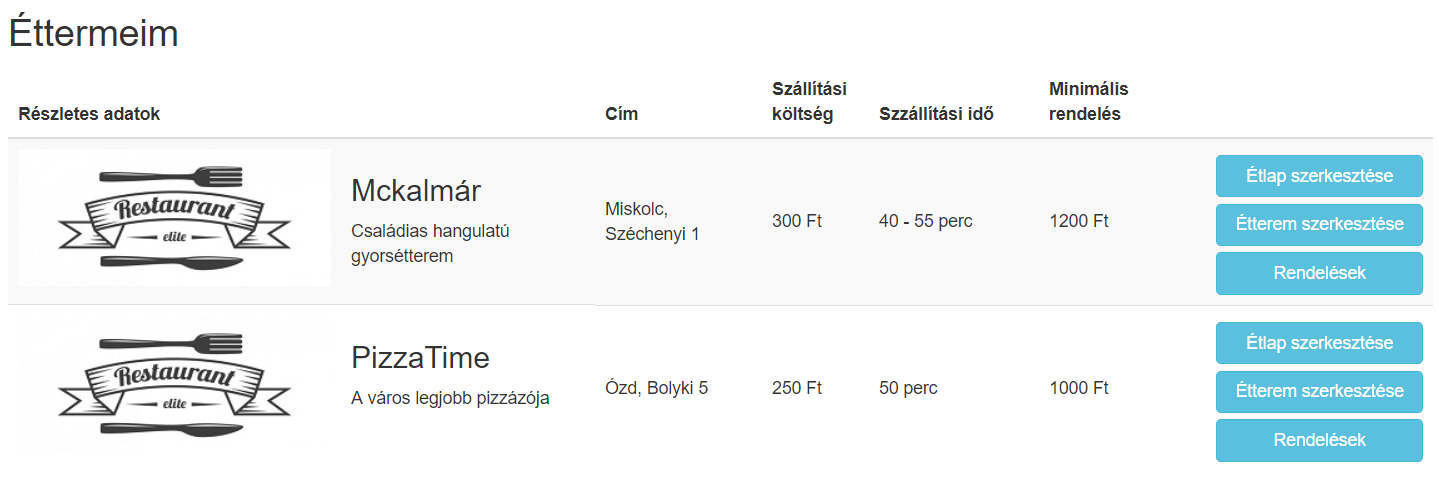
\includegraphics[scale=0.5]{kepek/my_restaurants.png}
\caption{A saját éttermek kilistázása}
\label{fig:my_restaurants}
\end{figure}

\subsection{Étlap szerkesztése}

Az étlap szerkesztése menüpont kiválasztása utána, egy táblázatot fogunk látni az adott étterem által forgalmazott ételekről és ezen ételek adatairól. Az elrendezés hasonló a user oldalon látott étlapok elrendezéséhez.

Az ételek egymás alatt, egy táblázatban jelennek meg. A táblázat egyes soraiban egy-egy étel szerepel, az oszlopaiban pedig az adott étel adatai. A táblázat jobb szélső oszlopában két gomb található, „Étel szerkesztése”, „Étel törlése”. A táblázat alatt egy „Étel felvitele” feliratú gomb van.

A táblázat felett egy legördülő menü van, amelynek segítségével a tulajdonos rá tud szűrni a különböző ételtípusokra, ezáltal könnyebben megtalálhatja a szerkeszteni, vagy törölni kívánt terméket. Az étel típus kiválasztása után, az ételek listája szűrve lesz az adott típus szerint, tehát csak a kívánt típusú ételek fognak megjelenni a táblázatban (\ref{fig:new_meal}. ábra).

\begin{figure}
\centering
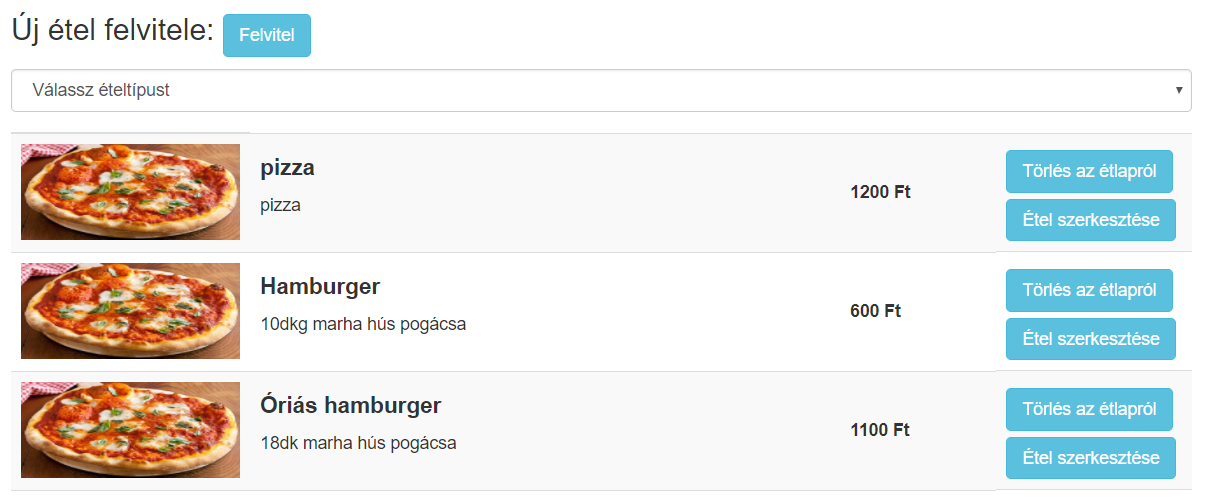
\includegraphics[scale=0.5]{kepek/new_meal.png}
\caption{Új étel hozzáadása}
\label{fig:new_meal}
\end{figure}

\subsection{Étel törlése}

Az étterem tulajdonosnak lehetősége van testre szabnia az étterme által biztosított kínáltaot. Vannak bizonyos ételek, melyeket csak szezonálisan lehet elkészíteni az alapszükségletük miatt, vagy csak valamilyen oknál fogva úgy dönt a vezetőség, hogy le kell kerülnie az étlapról. Ilyenkor van szükség az étel törlés funkcióra. Az „Étel törlése” gombra kattintva meghívásra kerül az étel törlése funkció, melynek hatására a kiválasztott étel törlődik a megjelenített ételek listájából, és törlődik az adatbázisból is.

\subsection{Étel szerkesztése}

Az étel szerkesztése funkcióval lehetőséget biztosítok az étterem tulajdonos számára, az étlapon szereplő termékek adatainak módosítására. Tehát ha egy adott ételnek megváltozik az ára vagy például az összetétele, akkor nem kell törölni azt, majd az új adatokkal ismét felvinni az adatbázisba. Mindössze rá kell kattintani a szerkeszteni kívánt termék sorában található gombok közül az „Étel szerkesztése” gombra, melynek hatására meghívódik az étel szerkesztése funkció.

Egy űrlapot fogunk látni, ahol a szükséges módosítások elvégzése után, a mentés gombbal lehet véglegesíteni a módosítást (\ref{fig:edit_meal}. ábra).

\begin{figure}
\centering
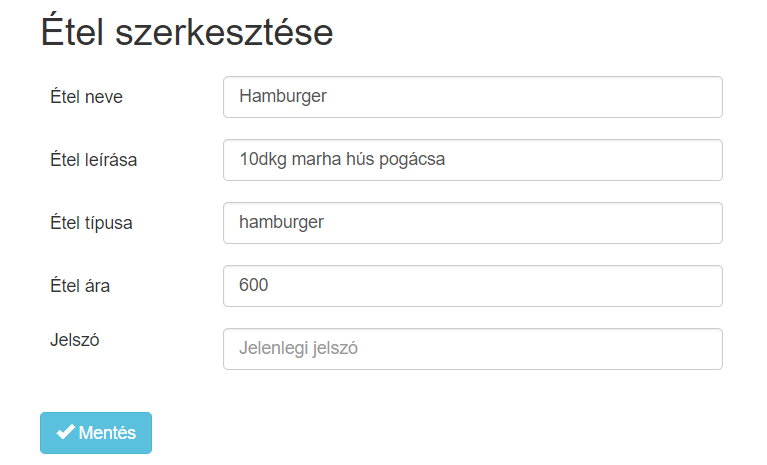
\includegraphics[scale=0.8]{kepek/edit_meal.png}
\caption{Egy étel adatainak szerkesztése}
\label{fig:edit_meal}
\end{figure}

\subsection{Étel felvitele}

Az étel felvitel gombra kattintva egy űrlap fog betöltődni. Az űrlap beviteli mezőkből áll, melyekkel az étlapra felvinni kívánt étel adatait tudjuk elküldeni a szervernek. Meg kell adni többek között az étel nevét, árát és típusát. Amennyiben minden szükséges mezőt kitöltöttünk a „Felvitel” gombra kattintva lehet véglegesíteni a műveletet.

\begin{figure}
\centering
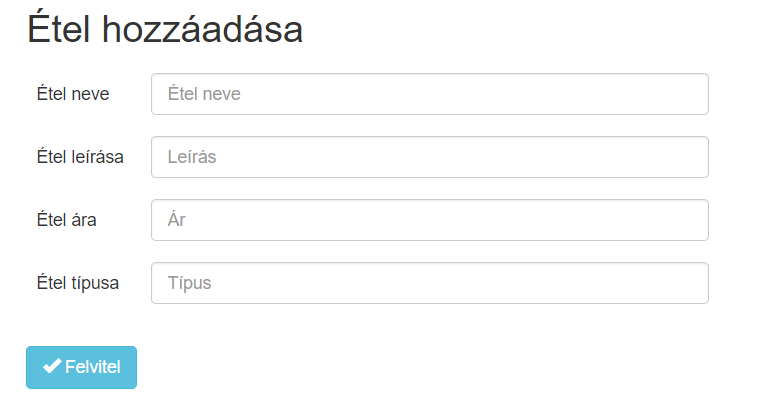
\includegraphics[scale=0.8]{kepek/add_meal.png}
\caption{Új étel felvitele az étlapra}
\label{fig:add_meal}
\end{figure}

\subsection{Rendelések}

Ahogy már említettem, az éttermeim funkció kilistázza a felhasználó adatbázisban szereplő éttermeit. Ilyenkor az éttermek táblázatos formában jelennek meg, minden étterem sorában szerepel egy „Rendelések” feliratú gomb. Erre a gombra kattintva a szerver kilistázza az adott étteremhez tartozó megrendeléseket, tehát azokat a rendeléseket, amiket ebben az étteremben adtak le a vásárlók. A rendelések táblázatos formában jelennek meg a felületen, egy sor egy rendelés. A táblázat oszlopaiban az egyes rendeléshez tartozó rendelési adatok vannak megjelenítve. Az adatok között szerepel a rendelő neve, rendelés időpontja, a megrendelt termékek, a rendelés összege és a fizetési módja.

\subsection{Étterem szerkesztése}

Egy étteremtulajdonosnak lehetősége lesz az éttermei adatainak módosítására. A szerkesztendő étterem sorában rá kell klikkelni az étterem szerkesztése gombra. Kattintás után megjelenik egy űrlap, amire fel kell vinni a módosítandó adatokat. Az adatok megadását követően a mentés gombbal lehet véglegesíteni a módosításokat (\ref{fig:edit_meal}. ábra).

\begin{figure}
\centering
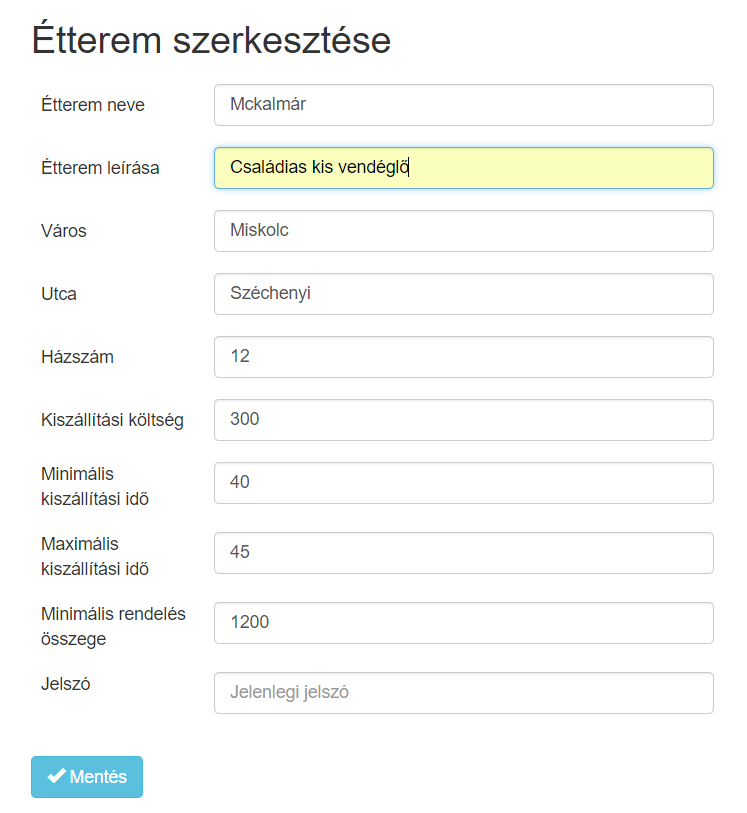
\includegraphics[scale=0.8]{kepek/edit_restaurant.png}
\caption{Étterem adatainak szerkesztése}
\label{fig:edit_restaurnt}
\end{figure}

\subsection{Étterem hozzáadása}

Egy étterem tulajdonosnak több étterme is lehet az adatbázisban. Az étterem hozzáadása menüpont alatt van lehetőség egy újabb éttermet felvinni. 
A menüpontra kattintva egy űrlapot fogunk látni, ahol a beviteli mezők egymás alatt helyezkednek el. Az egyes beviteli mezőkben az étterem különböző adatait lehet megadni. Az étterem nevét, leírását, címét. Ha elkészültünk az adatok megadásával, a „Felvitel” gombbal lehet véglegesíteni ezt a műveletet (\ref{fig:add_restaurant}. ábra).

\subsection{Profilom}

A profilom funkció az étterem tulajdonosok szempontjából is ugyanaz, mint a vásárlóknál. Kilistázza a bejelentkezett felhasználó adatait. Egy táblázatba foglalva kilistázza a felhasználó teljes nevét, felhasználónevét, email címét, telefonszámát és címét. A táblázat legalsó sorában van egy gomb „jelszó módosítása” felirattal.

A jelszó módosítás is ugyanúgy működik, mint a vásárlóknál. A „Jelszó módosítása” gombra kattintva megjelenik egy űrlap. Meg kell adni a jelenlegi jelszót, majd az új jelszót és végül meg kell erősíteni az új jelszót. A „Mentés” gombra kattintva megtörténik a jelszó cserélő funkció meghívása. Amennyibben a jelenlegi jelszó helyes, az új jelszó megfelel a kritériumoknak és megegyezik a megerősített jelszóval, megtörténik a jelszó módosítása.

\section{Megvalósítás AngularJS segítségével}

...
